\section{Component Loads Summary}\label{component-loads-summary}

Many building energy simulation programs provide reports that breakdown the design load into component contributions from walls, roofs, floors, underground walls, windows, interior walls, infiltration, ventilation, occupancy, lighting, refrigeration cases, and internal equipment. Some of these components have both sensible and latent subcomponents. It is important to understand the difference between gains and loads. ASHRAE Handbook of Fundamentals 2009 describes the space heat gain as ``...the rate at which heat enters into and/or is generated within a space'' while the space cooling load is ``the rate at which sensible and latent heat must be removed fro the space to maintain a constant space air temperature and humidity.''~ The difference is that the radiant heat gains which is ``absorbed by walls, floors, furniture, etc., contributed to the space cooling load only after a time lag.''

The heat balance algorithms used by EnergyPlus result in a single combined design load for a given zone and some, but not all, of the zone instantaneous heat gains. This section describes the estimation procedure for the three Component Loads Summary reports that shows an estimated breakdown of load components from each type of of heat gain for each zone. The three different reports are the Zone Component Loads Summary, the AirLoop Component Loads Summary and the Facility Component Loads Summary. The procedure described below is used for each zone and then the AirLoop and Facility level reports are generated by aggregating the results for the appropriate zones.

If the time of the peak load for each Zone for cooling exactly matches the time of the peak load for the AirLoop or Facility than the Estimated Cooling Peak Load Components will represent a sum of the values from the corresponding zones. Likewise the Estimated Heating Peak Load Components will add up for the AirLoop or Facility if the times of the heating peaks exactly match. This is not necessarily the case for Peak Conditions or the Engineering Checks tables. Since the sizing of Airloops is based on the system sizing they usually will be different than the sum of the corresonding zones. 

The Estimated Cooling Peak Load Components and Estimated Heating Peak Load Components subtables of the Zone Component Loads Summary report contain values that are estimated and are not part of the normal heat balance algorithms used in the rest of EnergyPlus.~ In particular, the column described as Sensible-Delayed represents an estimate of the sensible load contributed at the peak time based on radiant contributions from various load components that have radiant portions in previous timesteps. The focus of this section will be on the Sensible-Delayed column.

The columns labeled Sensible-Instant, Sensible-Return Air, and Latent are directly computed for people, lights, equipment, refrigeration, water use equipment,~ HVAC equipment losses, power generation equipment, infiltration, zone ventilation and interzone mixing. For example, Lights objects have inputs for the fractions of the gains that are to return air, radiant, visible and the remainder is convected.~ In this case, the fraction to return air is reported in the Sensible Return Air column and the fraction that is convected is reported in the Sensible-Instant column.

At the time of the peak load, each surface in the zone is contributing a convective heat loss or heat gain depending on the inside surface temperature.

The radiant portion of the internal heat gains from lighting, equipment, and incident solar are radiantly transmitted to the surfaces of the zone. The heat from these radiant gains is stored in the surfaces and retransmitted back into the zone over time as convective gains to the zone. By the time the heat is retransmitted, it is impossible to know the contribution of each possible radiant gain from past time steps on that surface into the convective gain for that timestep. The temperature change of the surface includes the impact of all of these radiant gains as well as any heat transfer through the surface.

To disaggregate the delayed affect of zone radiant (delayed) portions of the peak load, a pulse of radiant internal loads is used to determine custom radiant to convective decay curves for heating and cooling, essentially replicating part of the method used for Radiant Time Series (see Chapter 18 of ASHRAE Handbook of Fundamentals 2009) to isolate the delayed impacts of internal loads. This is performed during the zone sizing routines.

The response of each surface to a pulse of radiant heat is used to estimate the peak load components for solar gains and the radiant portion of internal gains. Subtracting these for each surface then leaves the peak load component from conduction through the surfaces. The approach is described in more detail below:

\begin{enumerate}
\def\labelenumi{\arabic{enumi})}
\item
  When zone sizing is performed for cooling or heating, the heat convected from each opaque surface for each timestep during sizing day is saved to an array.
\item
  For each type of internal gain, HVAC equipment gain, and solar energy entering the zone, the radiant and convective portions are saved for every timestep during sizing. In addition, for each type of radiant gain, the amount that lands on each surface in the zone is saved for evergy timestep during sizing.
\item
  An additional ``pulse sizing'' run is performed for cooling and heating during zone sizing that includes an additional small, single timestep, pulse of radiant-only heat for each zone but is otherwise the same as a normal zone sizing simulation. This is equivalent to adding an ElectricEquipment object that is scheduled for a single timestep and is 100\% radiant heat. The heat convected from each opaque surface for each timestep during sizing is saved to an array. This run is not used for sizing, but just to gather the impact of the pulse of radiant heat.
\item
  For each surface, a ``decay curve'' is developed by subtracting the results from the normal sizing (1) from the ``pulse'' sizing run (3). This represents the delay in converting incoming radiant heat into convected heat for each surface in the zone. The graphs below show the decay curves for an exterior wall (RIGHT-1) and an interior wall (SB23) for a test file.
\end{enumerate}

\begin{figure}[hbtp] % fig 343
\centering
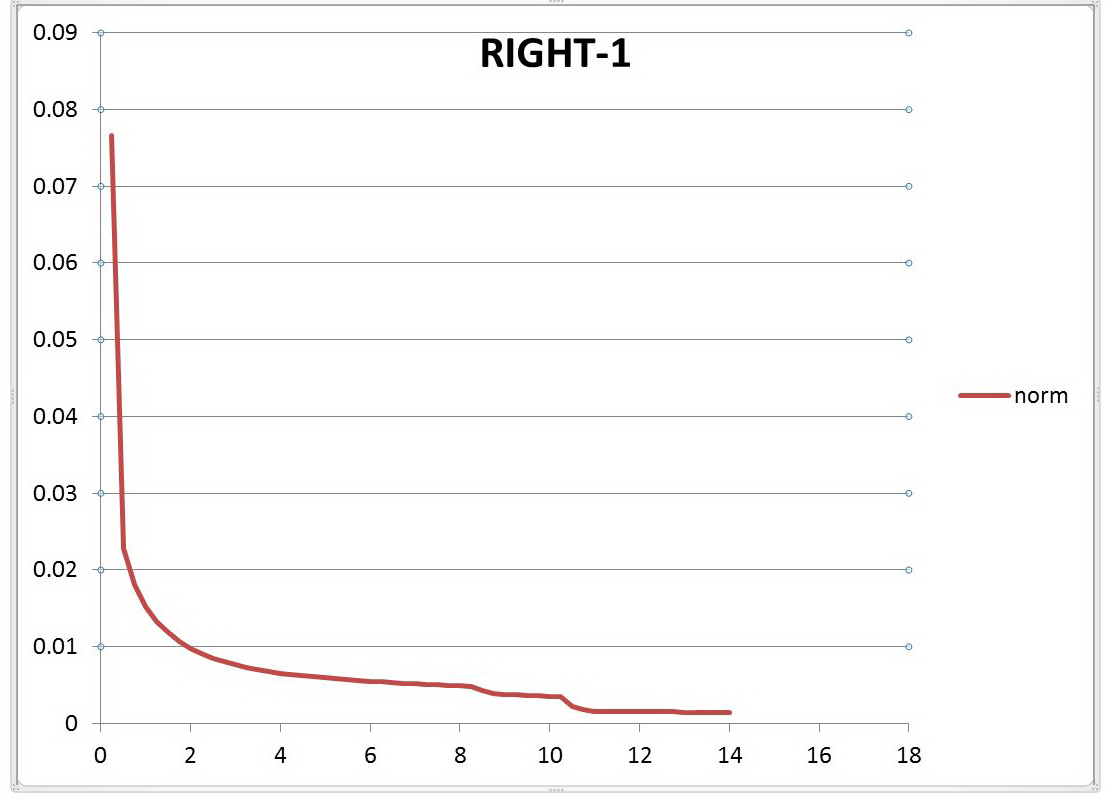
\includegraphics[width=0.9\textwidth, height=0.9\textheight, keepaspectratio=true]{media/image7912.png}
\caption{Load Component - Decay Curve of Exterior Wall \protect \label{fig:load-component-decay-curve-of-exterior-wall}}
\end{figure}

\begin{figure}[hbtp] % fig 344
\centering
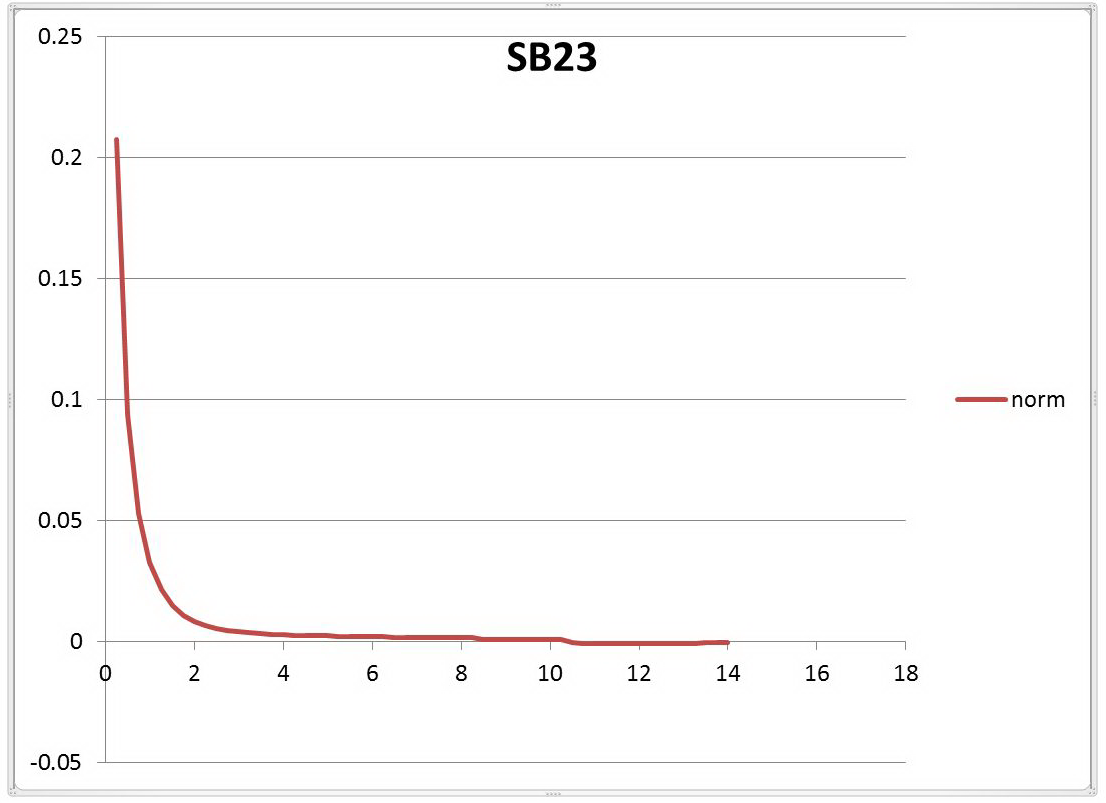
\includegraphics[width=0.9\textwidth, height=0.9\textheight, keepaspectratio=true]{media/image7913.png}
\caption{Load Component - Decay Curve of Interior Wall \protect \label{fig:load-component-decay-curve-of-interior-wall}}
\end{figure}

\begin{enumerate}
\def\labelenumi{\arabic{enumi})}
\setcounter{enumi}{4}
\item
  Using the internal and solar gain results saved from the normal sizing period in step (2), for each timestep prior to and including the time of the peak load during the sizing day, the decay curve is applied to each radiant gain on each surface for each timestep to generate a predicted delayed load component for the internal and solar gains for each timestep that comprise the peak load (based on Timesteps in Averaging Window). Timesteps just before the peak have much larger impacts than those just a few timesteps before the peak.~ These results will be the radiant portion of the load for each type of internal and solar gain.
\item
  The difference between the sum of the predicted convective loads from internal and solar gains from step (5) and the total convective loads for that surface for the timesteps that comprise the peak load from step (1) is assumed to be the load from heat transfer through that surface.~ This is essentially subtracting out the radiant portions of the internal and solar gains on each surface for the sizing day.
\end{enumerate}

\subsection{Estimated Component Load Details}\label{estimated-component-load-details}

In HeatBalanceInternalHeatGains, in the InitInternalHeatGains routine, the single timestep pulse is added to the thermal radiation absorbed on the inside surface. It is based on 0.01 W per square meter of the zone area. The time of the pulse and the amount received by each surface is also saved. A new routine GatherComponentLoadsIntGain was also added to that file that gathers the instantenous heat gains from people, lights, equipment, refrigeration equipment, water use, hvac losses, and power generation. Latent gains from people and refrigeration are also gathered along with the radiant portion of the gains from these same sources. EnergyPlus tracks internal gains by type, and these are grouped as follows for the rows of the report:

The gains from ``People'' contain:

\begin{itemize}
\tightlist
\item
  IntGainTypeOf\_People
\end{itemize}

The gains from ``Lights'' contain:

\begin{itemize}
\tightlist
\item
  IntGainTypeOf\_Lights
\end{itemize}

The gains from ``Equipment'' contain:

\begin{itemize}
\item
  IntGainTypeOf\_ElectricEquipment
\item
  IntGainTypeOf\_ElectricEquipmentITEAirCooled
\item
  IntGainTypeOf\_GasEquipment
\item
  IntGainTypeOf\_HotWaterEquipment
\item
  IntGainTypeOf\_SteamEquipment
\item
  IntGainTypeOf\_OtherEquipment
\end{itemize}

The gains from ``Refrigeration'' contain:

\begin{itemize}
\item
  IntGainTypeOf\_RefrigerationCase
\item
  IntGainTypeOf\_RefrigerationCompressorRack
\item
  IntGainTypeOf\_RefrigerationSystemAirCooledCondenser
\item
  IntGainTypeOf\_RefrigerationSystemSuctionPipe
\item
  IntGainTypeOf\_RefrigerationSecondaryReceiver
\item
  IntGainTypeOf\_RefrigerationSecondaryPipe
\item
  IntGainTypeOf\_RefrigerationWalkIn
\item
  IntGainTypeOf\_RefrigerationTransSysAirCooledGasCooler
\item
  IntGainTypeOf\_RefrigerationTransSysSuctionPipeMT
\item
  IntGainTypeOf\_RefrigerationTransSysSuctionPipeLT
\end{itemize}

The gains from ``Water Use Equipment'' contain:

\begin{itemize}
\item
  IntGainTypeOf\_WaterUseEquipment
\item
  IntGainTypeOf\_WaterHeaterMixed
\item
  IntGainTypeOf\_WaterHeaterStratified
\end{itemize}

The gains from ``HVAC Equipment Losses'' which are gains to the zone due to the location of the equipment within the zone include:

\begin{itemize}
\item
  IntGainTypeOf\_ZoneBaseboardOutdoorTemperatureControlled
\item
  IntGainTypeOf\_ThermalStorageChilledWaterMixed
\item
  IntGainTypeOf\_ThermalStorageChilledWaterStratified
\item
  IntGainTypeOf\_PipeIndoor
\item
  IntGainTypeOf\_Pump\_VarSpeed
\item
  IntGainTypeOf\_Pump\_ConSpeed
\item
  IntGainTypeOf\_Pump\_Cond
\item
  IntGainTypeOf\_PumpBank\_VarSpeed
\item
  IntGainTypeOf\_PumpBank\_ConSpeed
\item
  IntGainTypeOf\_PlantComponentUserDefined
\item
  IntGainTypeOf\_CoilUserDefined
\item
  IntGainTypeOf\_ZoneHVACForcedAirUserDefined
\item
  IntGainTypeOf\_AirTerminalUserDefined
\item
  IntGainTypeOf\_PackagedTESCoilTank
\item
  IntGainTypeOf\_FanSystemModel
\item
  IntGainTypeOf\_SecCoolingDXCoilSingleSpeed
\item
  IntGainTypeOf\_SecHeatingDXCoilSingleSpeed
\item
  IntGainTypeOf\_SecCoolingDXCoilTwoSpeed
\item
  IntGainTypeOf\_SecCoolingDXCoilMultiSpeed
\item
  IntGainTypeOf\_SecHeatingDXCoilMultiSpeed
\end{itemize}

The gains from ``Power Generation Equipment'' include:

\begin{itemize}
\item
  IntGainTypeOf\_GeneratorFuelCell
\item
  IntGainTypeOf\_GeneratorMicroCHP
\item
  IntGainTypeOf\_ElectricLoadCenterTransformer
\item
  IntGainTypeOf\_ElectricLoadCenterInverterSimple
\item
  IntGainTypeOf\_ElectricLoadCenterInverterFunctionOfPower
\item
  IntGainTypeOf\_ElectricLoadCenterInverterLookUpTable
\item
  IntGainTypeOf\_ElectricLoadCenterStorageBattery
\end{itemize}

The ReportSurfaceHeatBalance routine in the HeatBalanceSurfaceManger module gathers the shortwave radiant heat gain from lighting and fenestration solar gains on each surface. In the same module, the CalcHeatBalanceInsideSurf routine gathers the surface by surface convection for both the normal and pulse zone sizing times along with the net radiation on the surface during the normal zone sizing times. In addition, a routine called GatherComponentLoadSurfAbsFact gathers the factors used in distributing the radiant heat from a zone to each surface (TMULT and ITABSF).

The SizingManager module repeats the zone sizing portion of the procedure when this report is requested.~ The pulse occurs at 10am during the zone sizing simulations. The 10am time was chosen after some testing that looked at pulses at different times of the day. It is ~important that the pulse occurs while the system is running and stable not during start up hours. In addition, the plus timing needs to be early enough that the duration of the resulting decay curve can be appropriate applied to as many timesteps as possible during the peak day.

The following subroutines in the OutputReportTabular module produce the report:

\begin{itemize}
\item
  ComputeLoadComponentDecayCurve
\item
  GatherComponentLoadsSurface
\item
  GatherComonentLoadsHVAC
\item
  WriteLoadComponentSummaryTables
\item
  GetDelaySequences
\item
  MovingAvgAtMaxTime
\item
  ComputeTableBodyUsingMovingAvg
\end{itemize}

The ComputeLoadComponentDecayCurve routine determines the heating and cooling decay curves using the following (for cooling but repeated also for heating):

\begin{lstlisting}
  TimeOfPulse = radiantPulseTimestep(ZoneNum,CoolDesSelected)
  DO TimeStep = TimeOfPulse, NumOfTimeStepInHour* 24
    IF (radiantPulseReceived(surfNum,CoolDesSelected) .NE. 0.0) THEN
      diff = loadConvectedWithPulse(surfNum,TimeStep,CoolDesSelected)
           - loadConvectedNormal(surfNum,TimeStep,CoolDesSelected)
      decayCurveCool(surfNum, TimeStep - TimeOfPulse + 1) = -diff /
          radiantPulseReceived(surfNum,CoolDesSelected)
    ELSE
      decayCurveCool(surfNum, TimeStep - TimeOfPulse + 1) = 0.0
    END IF
  END DO
\end{lstlisting}

The ComputeTableBodyUsingMovingAvg routine applies the decay curve to the load components. It does the following for the heating and cooling sizing period that was selected and for each zone and each surface in the zone

\begin{enumerate}
\def\labelenumi{\alph{enumi}.}
\item
  Determine the heat gain on the surface of people, equipment, hvac losses, power generation and long wave light radiation.
\item
  For each time step backwards from the current timestep, estimate the delayed convected heat from people, equipment, HVAC losses, power generation, lighting long wave radiation, lighting short wave radiation, and fenestration solar by multiplying the decay curve with the value determined from (a).
\item
  Accumulate the values on a zone basis
\item
  Determine the remaining convective heat from surfaces that are not from these gains and remove the net surface radiation (output variable Surface Inside Face Convection Heat Gain Rate)
\item
  Store the estimated values in a sequence to be later averaged over the averaging window.
\end{enumerate}
